\section{Apêndice}

\subsection{Memorial de cálculo}

A norma NOR.DISTRIBU-ENGE-0022 de Fornecimento de Energia Elétrica à Edificações com Múltiplas Unidades Consumidoras foi utilizada como base para o cálculo da demanda da edificação do tipo prédio de escritórios.

Para simplificação dos cálculos o fator de potêncoa dos eletrodomésticos foi determinada como 0.92, exceto para equipamentos notadamente resistivos.

A parcela "a" para a soma das demandas diz respeito à iluminação e tomadas de uso geral e tem como base o Quadro 4 da norma supracitada.
    
Para escritórios deve-se aplicar um fator de demanda de 100\% para os primeiros 20 kVA e 70\% para o excedente de 20 kVA.
    
    
\begin{table}[H]
\centering
\caption{Cálculo da parcela "a" da demanda}
\begin{tabular}{|c|c|c|c|l}
\cline{1-4}
\textbf{Descrição} & \textbf{Potência (kW)} & \textbf{F.P.} & \textbf{Potência (kVA)} &  \\ \cline{1-4}
Iluminação         & 40                     & 1             & 40                      &  \\ \cline{1-4}
TUG                & 75                     & 0,92          & 81,52                    &  \\ \cline{1-4}
\textbf{TOTAL}     & \textbf{115}           & \textbf{}     & \textbf{121,52}          &  \\ \cline{1-4}
\end{tabular}
\end{table}
    
Dessa forma, a demanda para esta parcela é:

\begin{center}
    $Da = 100\% \times 20 \, \text{kVA} + 70\% \times 101.52 \, \text{kVA} = 91.06 \, \text{kVA}$
\end{center}

E a potência instalada:

\begin{center}
    $Pa = 115 \, \text{kW}$
\end{center}

A parcela "b", $b=b1+b2+b3+b4+b5+b6$ representa a soma das demandas dos aparelhos eletrodomésticos e de aquecimento. Referente a essa parcela, a contribuição do quadro de cargas diz respeito apenas à subparcela "b2" que diz respeito a aquecedores de água com potência superior a 1 kVA de acordo com o Quadro 5 da norma. Para cerca de 10 aquecedores o fator de demanda é de 60\%.

\begin{table}[H]
\centering
\caption{Cálculo da parcela "b" da demanda}
\begin{tabular}{|c|c|c|c|c|c|}
\hline
\textbf{QTDA} & \textbf{UND} & \textbf{Descrição} & \textbf{Potência (kW)} & \textbf{F.P.} & \textbf{Potência (kVA)} \\ \hline
10            & und          & Aquecedores        & 50                     & 1             & 50                      \\ \hline
\multicolumn{3}{|l|}{\textbf{TOTAL}}              & \textbf{50}            & \textbf{}     & \textbf{50}             \\ \hline
\end{tabular}
\end{table}

Dessa forma, a demanda para esta parcela é:

\begin{center}
    $Db = 60\% \times 50 \, \text{kVA} = 30 \, \text{kVA}$
\end{center}

E a potência instalada:

\begin{center}
    $Pb = 50 \, \text{kW}$
\end{center}

A terceira parcela "c" representa a demanda dos aparelhos de ar condicionado calculada
aplicando-se os fatores de demanda do Quadro 7, e como são 24 aparelhos, o fator de demanda será de 80\%. 

\begin{table}[H]
\centering
\caption{Cálculo da parcela "c" da demanda}
\begin{tabular}{|c|c|c|c|c|c|c|}
\hline
\textbf{QTDA} & \textbf{UND} & \textbf{P. UNID. (W)} & \textbf{Descrição}                                                    & \textbf{\begin{tabular}[c]{@{}c@{}}Potência \\ (kW)\end{tabular}} & \textbf{F.P.} & \textbf{\begin{tabular}[c]{@{}c@{}}Potência \\ (kVA)\end{tabular}} \\ \hline
5             & und          & 3.500                 & \begin{tabular}[c]{@{}c@{}}Ar Condicionado \\ 12.000 BTU\end{tabular} & 17,5                                                              & 0,92          & 19,02                                                              \\ \hline
10            & und          & 5.300                 & \begin{tabular}[c]{@{}c@{}}Ar Condicionado \\ 18.000 BTU\end{tabular} & 53                                                                & 0,92          & 57,61                                                              \\ \hline
6             & und          & 8.800                 & \begin{tabular}[c]{@{}c@{}}Ar Condicionado \\ 30.000 BTU\end{tabular} & 52,8                                                              & 0,92          & 57,39                                                              \\ \hline
3             & und          & 17.600                & \begin{tabular}[c]{@{}c@{}}Ar Condicionado \\ 60.000 BTU\end{tabular} & 52,8                                                              & 0,92          & 57,39                                                              \\ \hline
\multicolumn{4}{|l|}{\textbf{TOTAL}}                                                                                         & \textbf{176,1}                                                    & \textbf{}     & \textbf{191,41}                                                    \\ \hline
\end{tabular}
\end{table}

Dessa forma, a demanda para esta parcela é:

\begin{center}
    $Dc = 80\% \times 191.41 \, \text{kVA} = 153.13 \, \text{kVA}$
\end{center}

E a potência instalada:

\begin{center}
    $Pc = 176.1 \, \text{kW}$
\end{center}

A parcela "d" representa a demanda dos motores monofásicos e trifásicos calculada utilizando-se os valores dos Quadros 8 e 9. No caso deste projeto, será usado apenas o Quadro 9 que diz respeito a motores trifásicos e os dados extraídos para motores trifásicos de 3cv, 5cv e 10cv estão apresentados na tabela abaixo.

% 3cv -> P = 2.87kW -> FP = 0.61
% 5cv -> P = 4.33kW -> FP = 0.64
% 10cv -> P = 8.56kW -> FP = 0.62
\begin{table}[H]
\centering
\caption{Cálculo da parcela "d" da demanda}
\begin{tabular}{|c|c|c|c|c|c|c|}
\hline
\textbf{QTDA} & \textbf{UND} & \textbf{P. UNID. (W)} & \textbf{Descrição}                                               & \textbf{\begin{tabular}[c]{@{}c@{}}Potência \\ (kW)\end{tabular}} & \textbf{F.P.} & \textbf{\begin{tabular}[c]{@{}c@{}}Potência \\ (kVA)\end{tabular}} \\ \hline
2             & und          & 2.870                 & \begin{tabular}[c]{@{}c@{}}Motor Trifásico \\ 3 cv\end{tabular}  & 5,74                                                              & 0,61          & 9,41                                                               \\ \hline
6             & und          & 4.330                 & \begin{tabular}[c]{@{}c@{}}Motor Trifásico \\ 5 cv\end{tabular}  & 25,98                                                             & 0,64          & 40,59                                                              \\ \hline
4             & und          & 8.560                 & \begin{tabular}[c]{@{}c@{}}Motor Trifásico \\ 10 cv\end{tabular} & 34,24                                                             & 0,62          & 55,23                                                              \\ \hline
\multicolumn{4}{|l|}{\textbf{TOTAL}}                                                                                    & \textbf{65,96}                                                    & \textbf{}     & \textbf{105,23}                                                    \\ \hline
\end{tabular}
\end{table}

Dessa forma, a demanda para esta parcela é:

\begin{center}
    $Dd = 105.23 \, \text{kVA}$
\end{center}

E a potência instalada:

\begin{center}
    $Pd = 65.96 \, \text{kW}$
\end{center}

Em relação a previsão de carga para futuras expansões de 100 kW, foi atribuído um fator de potência de 0.8, justificado como a média entre futuras cargas que podem ter natureza motora ou resistiva. Assim, resultando em um demanda de $Dexp = 125 \, \text{kVA}$ e potência instalada de $Pexp = 100 \, \text{kW}$

Portanto, a carga total instalada em kW será de:

\begin{center}
    $Ct = Pa + Pb + Pc + Pd + Pexp = 507.08 \, \text{kW}$
\end{center}

E a demanda total em kVA:

\begin{center}
    $Dt = Da + Db + Dc + Dd + Dexp = 504.4 \, \text{kVA}$
\end{center}

A corrente máxima prevista será:

\begin{center}
    $I_{max} = \frac{Dt}{V_{MT} \sqrt{3}} = \frac{504.4 \times 10^3}{13.8 \times 10^3 \times \sqrt{3}} = 21.103 \, \text{A}$
\end{center}

\subsection{Desenhos estruturais}

\begin{figure}[H] 
\centering
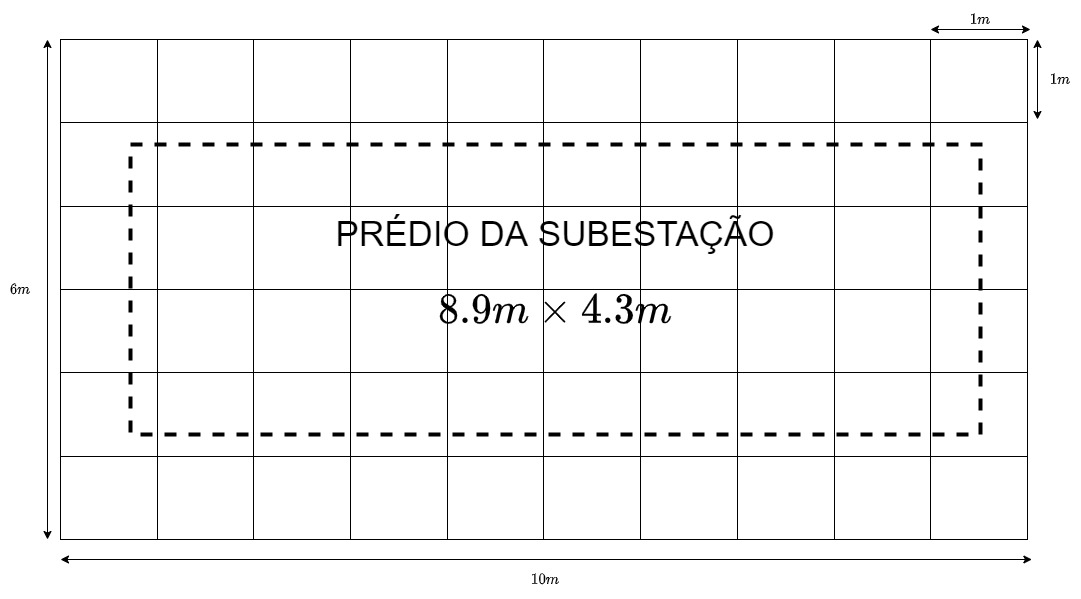
\includegraphics[width=16cm]{Imagens/malha_aterramento.jpg}
\caption{Desenho estrutural da malha de aterramento proposta.}
\label{malha_terra} 
\end{figure}

\newpage

\vspace{60pt}
\begin{figure}[htbp!]
    \centering
    \vspace{10cm}
		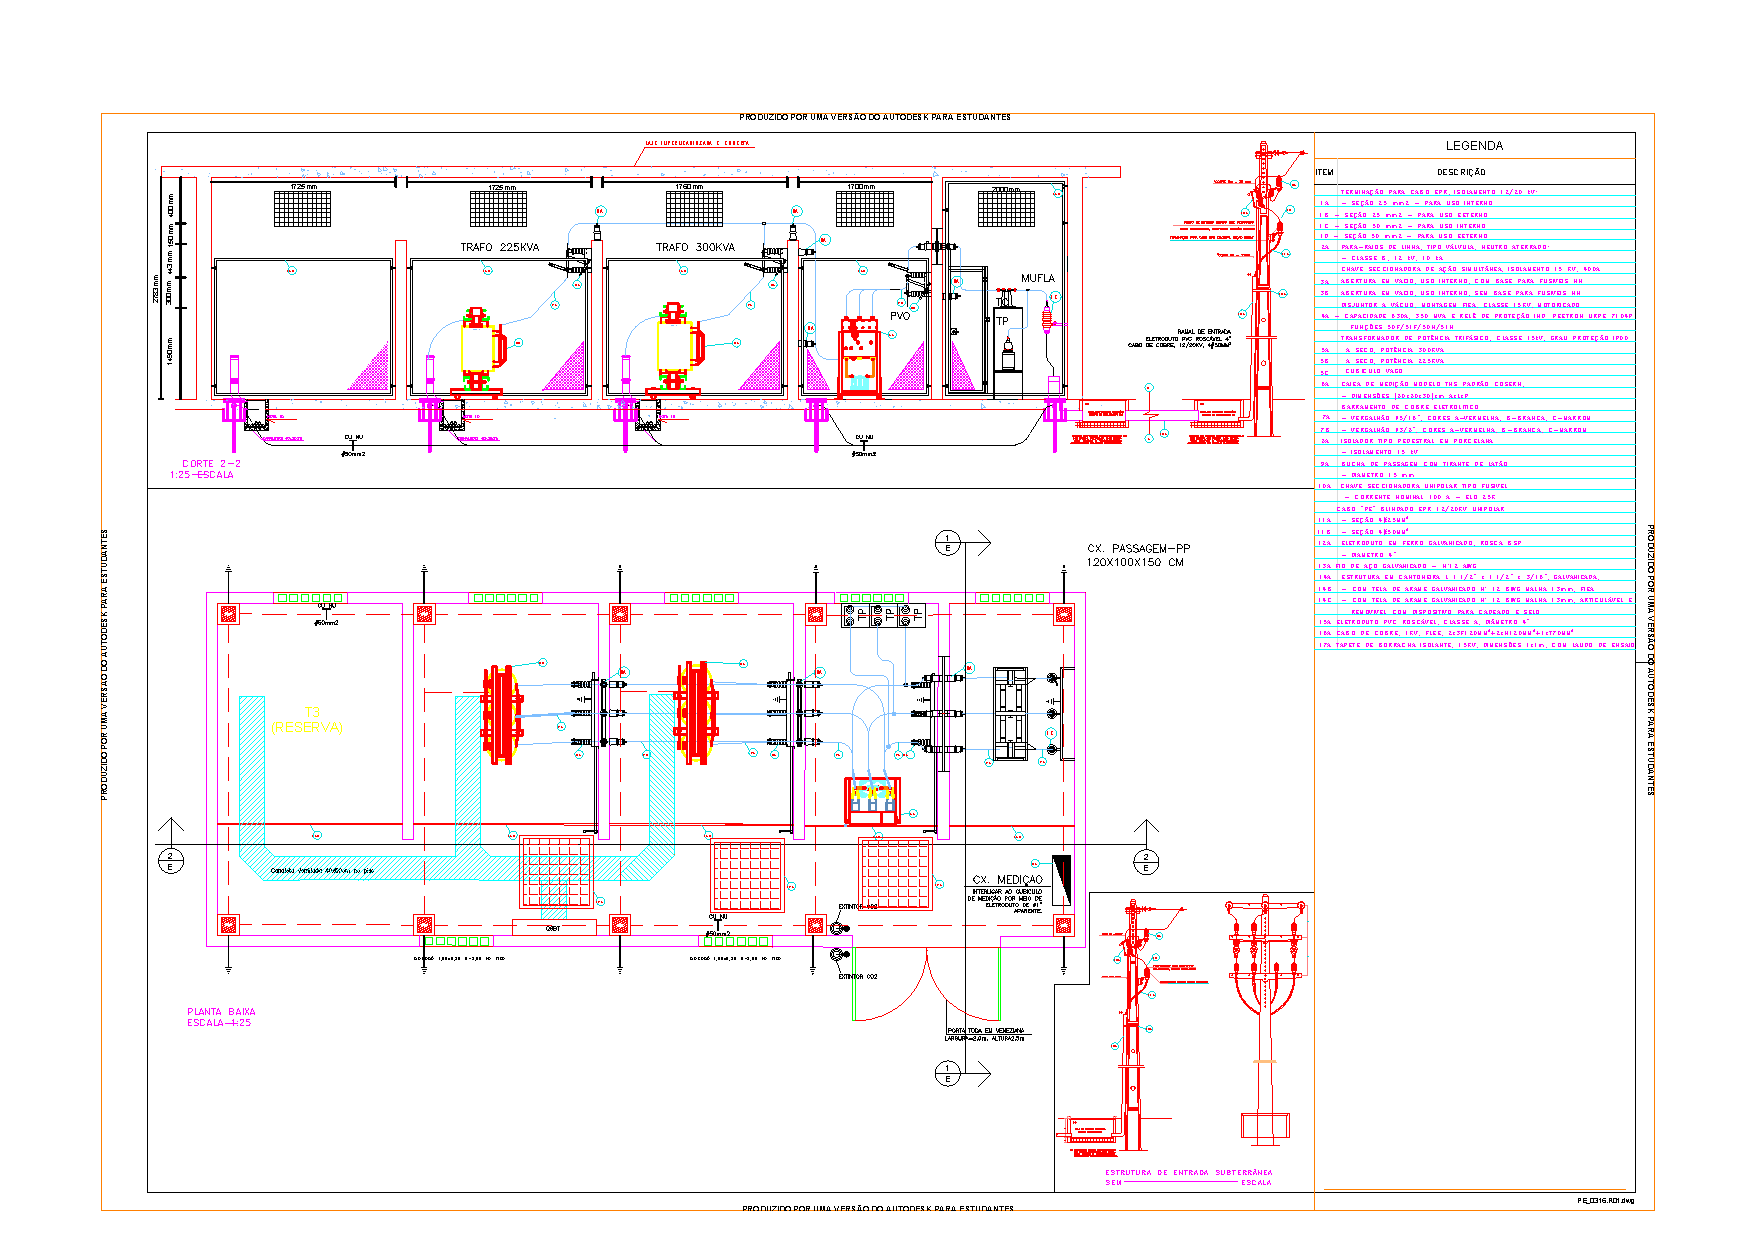
\includepdf[page={1},angle=270, width=18cm]{subestacao1.pdf}  
	%\caption{Desenhos indicativos das estruturas da subestação, parte 1.}
	\label{se:1}
\end{figure}

\newpage

\vspace{60pt}
\begin{figure}[htbp!]
    \centering
    \vspace{10cm}
		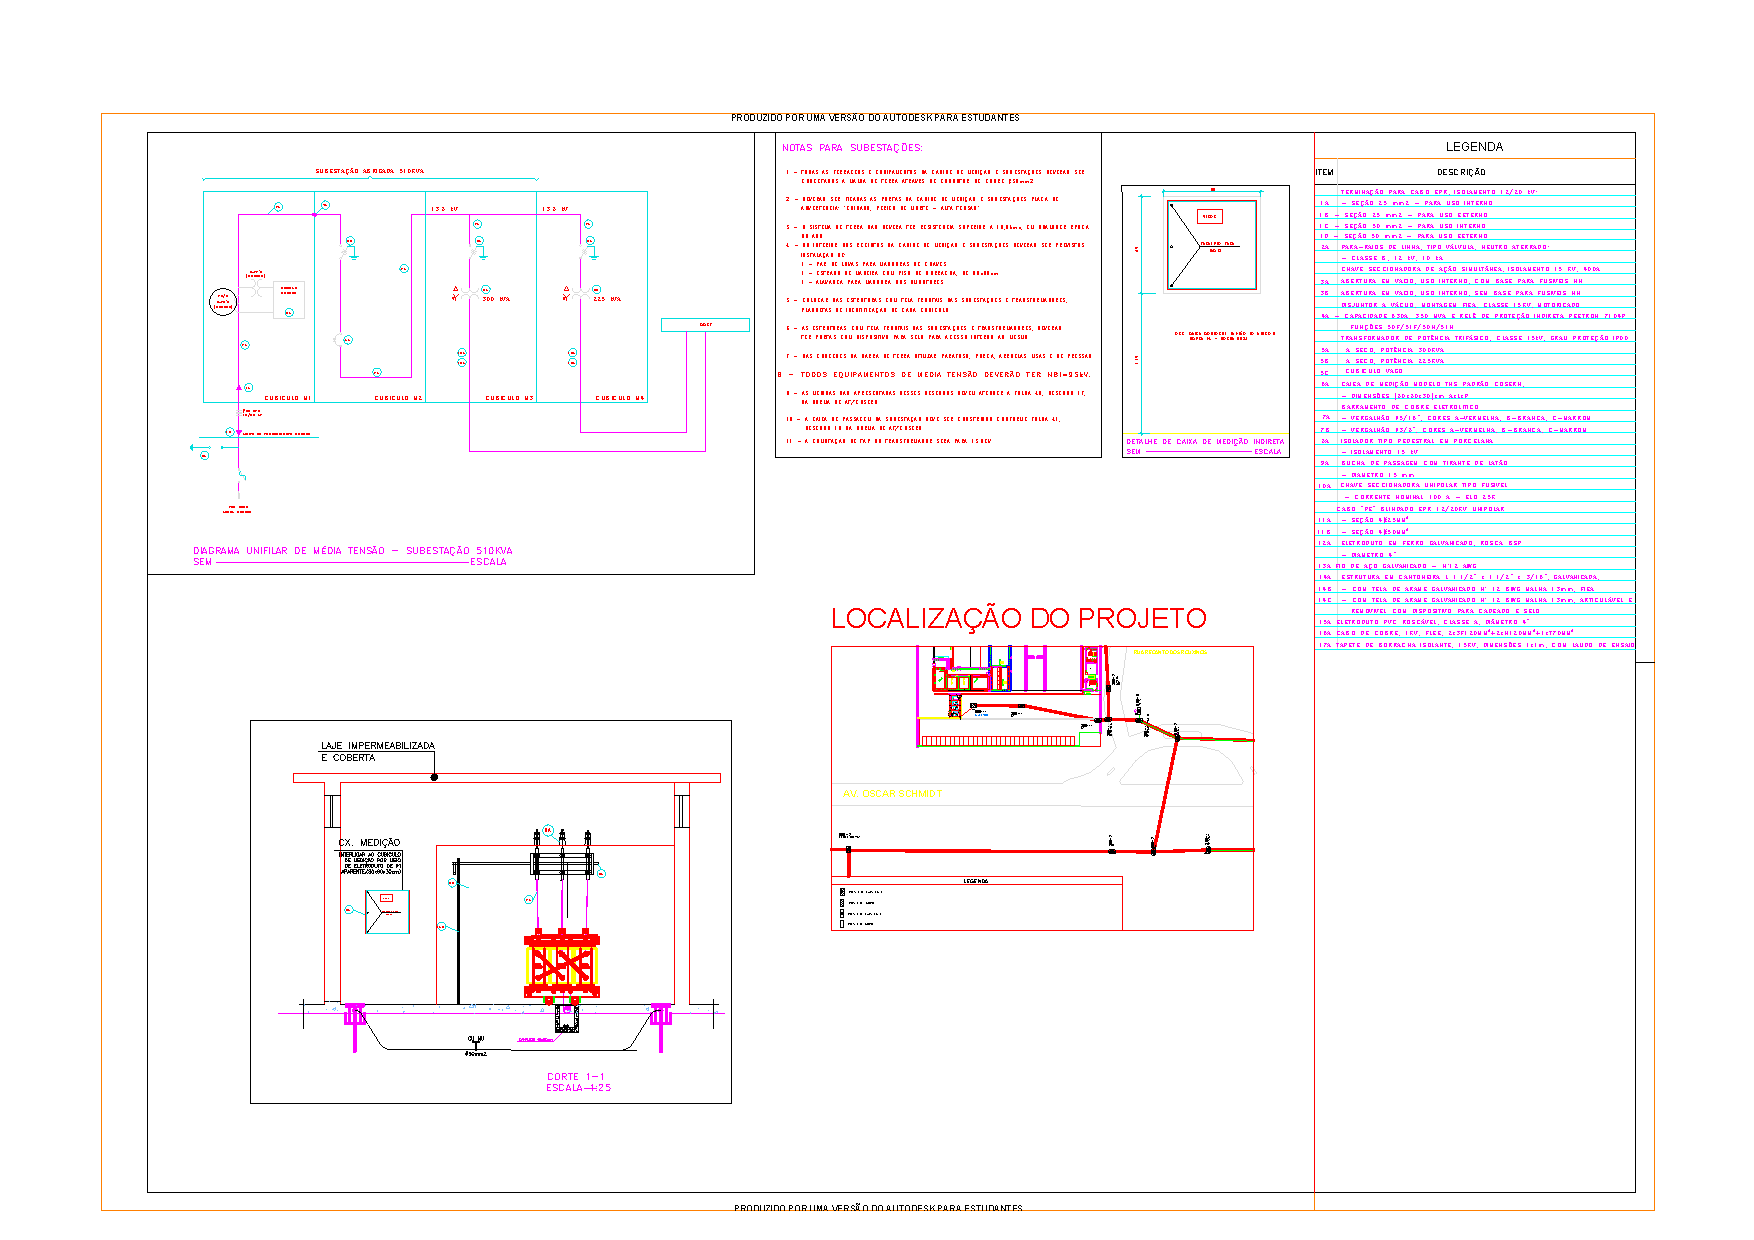
\includepdf[page={1},angle=270, width=18cm]{subestacao2.pdf}  
	%\caption{Desenhos indicativos das estruturas da subestação, parte 1.}
	\label{se:2}
\end{figure}

\newpage

%\section{Anexo}

%\begin{figure}[H] 
%\centering
%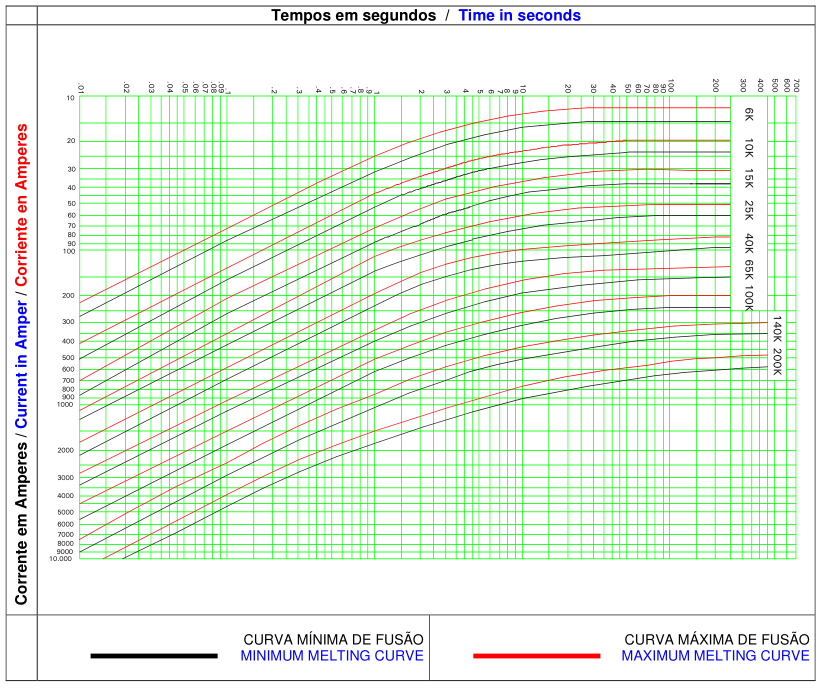
\includegraphics[width=16cm]{Imagens/curva_fusao.png}
%\caption{Curva mínima e máxima de fusão do elo fusível do fabricante Hubbell com foco no elo 25K. Fonte: \cite{elofusivel}}
%\label{curva_fusao} 
%\end{figure}

\newpage

\vspace{60pt}
\begin{figure}[htbp!]
    \centering
    \vspace{10cm}
		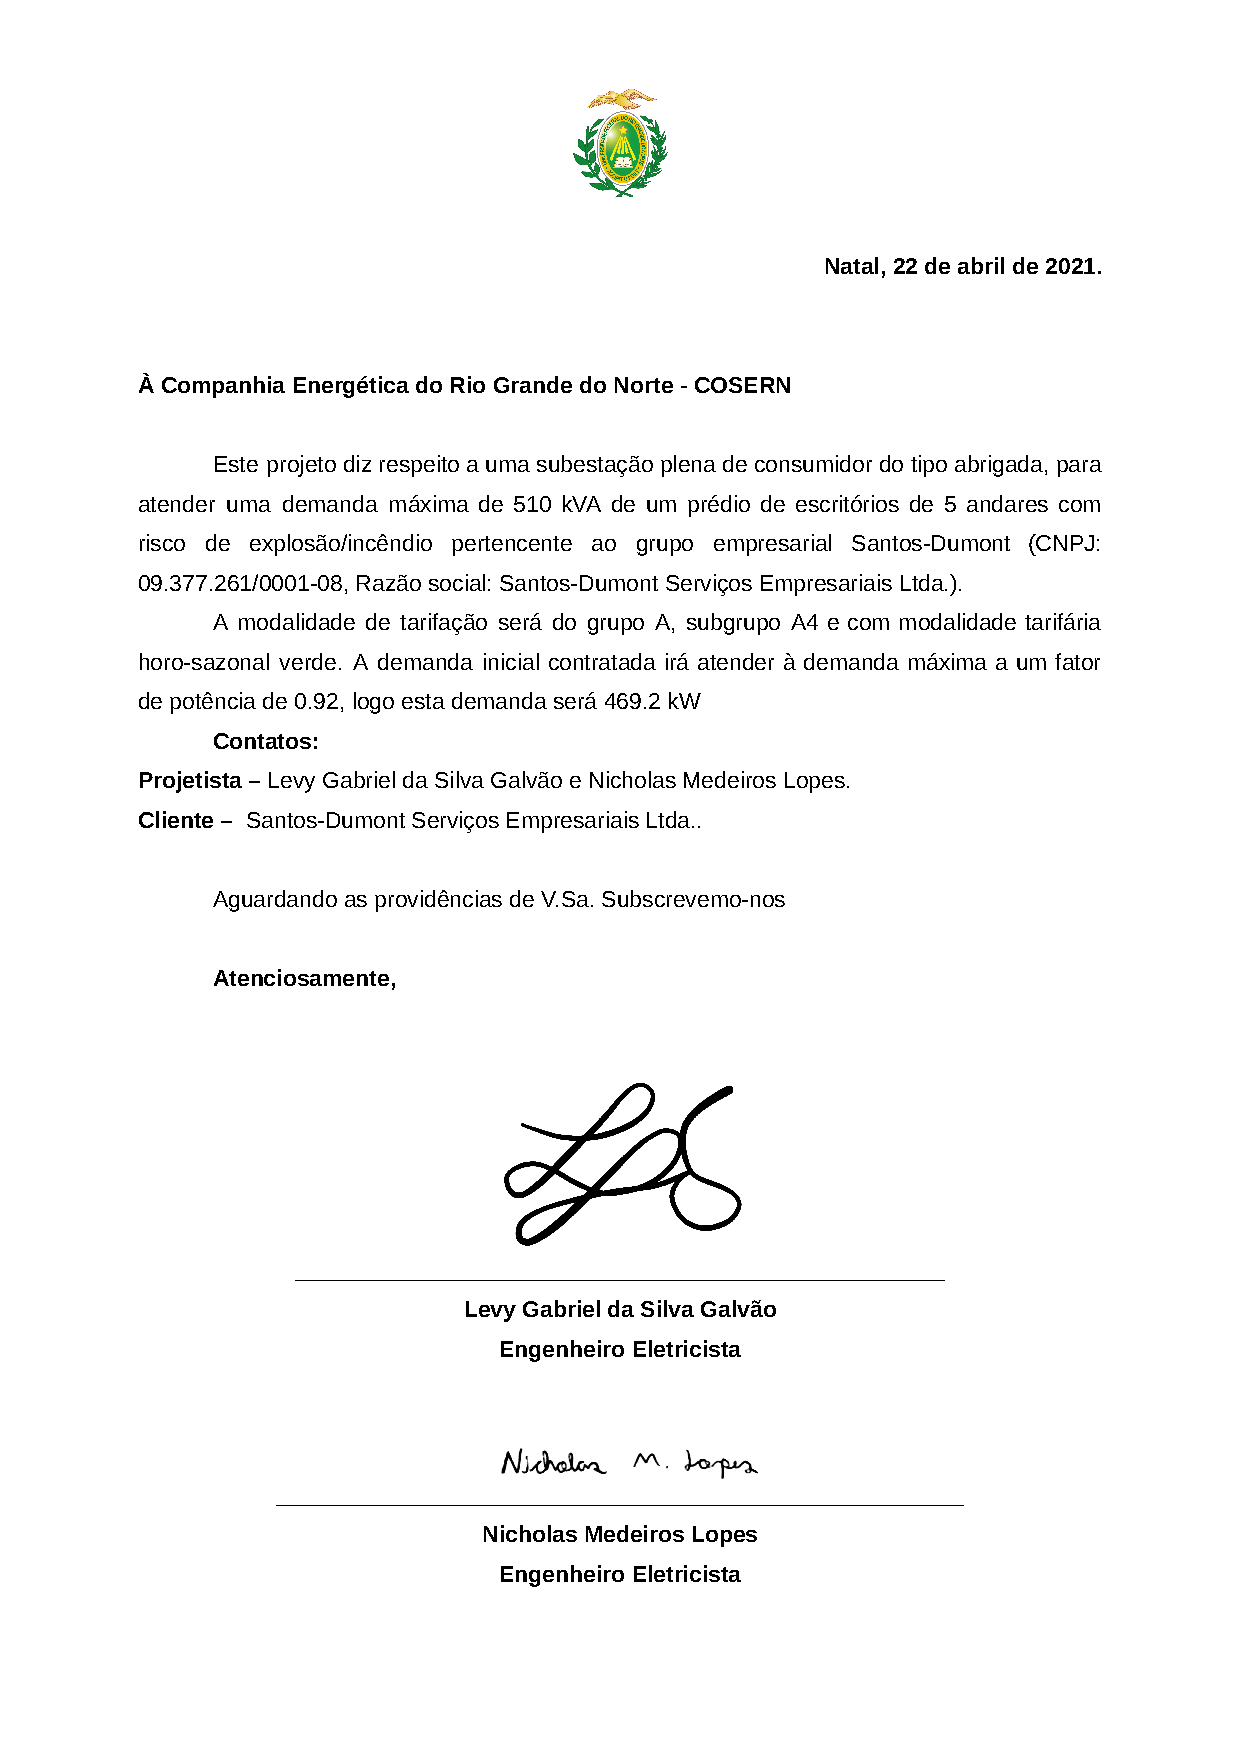
\includepdf[page={1} width=18cm]{carta.pdf}  
	%\caption{Desenhos indicativos das estruturas da subestação, parte 1.}
	\label{carta}
\end{figure}

\newpage